%%%%%%%%%%%%%%%%%%%%%%%%%%%%%%%%%%%%%%%%%%%%%%%%%%%%%%%%%%%%%%%%%%%%%%
% How to use writeLaTeX: 
%
% You edit the source code here on the left, and the preview on the
% right shows you the result within a few seconds.
%
% Bookmark this page and share the URL with your co-authors. They can
% edit at the same time!
%
% You can upload figures, bibliographies, custom classes and
% styles using the files menu.
%
%%%%%%%%%%%%%%%%%%%%%%%%%%%%%%%%%%%%%%%%%%%%%%%%%%%%%%%%%%%%%%%%%%%%%%

\documentclass[12pt]{article}

\usepackage{sbc-template}

\usepackage{graphicx,url}
\usepackage{algorithm}
\usepackage{algpseudocode}

%\usepackage[brazil]{babel}   
\usepackage[utf8]{inputenc}  

     
\sloppy

% (i) .pdf (gerado a partir do latex)  do relatório do trabalho de, no máximo, 10 páginas. Páginas adicionais serão descontadas em 2 pontos por página excendente da nota que foi alcançada.

% Você devera entregar alem dos codigos implementados, um relat orio (obrigatoriamente feito em TeX) em formato PDF (juntamente com seus códigos-fontes em TeX) descrevendo detalhes das implementações, dos experimentos e resultados obtidos.

\title{Arborescência}

\author{Caio Henrique Alvarenga Gonçalves\inst{1}, Daniel Valadares de Souza Felix\inst{1}, \\ Gustavo Silvestre Almeida Conceição\inst{1}, João Vitor Lima de Melo\inst{1}, \\ Larissa Valadares Silqueira\inst{1}, Leonardo Barbosa Brandão\inst{1} }

\address{Instituto de Ciências Exatas e Informática \\ Pontifícia Universidade Católica de Minas Gerais (PUC Minas)
{}
}

\begin{document} 

\maketitle
     
\begin{resumo} 
  Este artigo explora a implementação de dois algoritmos para a resolução do problema da arborescência mínima em grafos direcionados, seguindo as abordagens propostas por Edmonds e Tarjan. No relatório, é detalhado o funcionamento desses métodos, apresentando simulações realizadas com grafos direcionados diversos. Também é realizada uma análise dos resultados dos experimentos e uma comparação dos custos computacionais dos algoritmos. Com isso, se oferece uma visão abrangente desses métodos, destacando suas eficiências e desempenhos em cenários variados de grafos direcionados.

  \textbf{Palavras-Chave:} Arborescência, Edmonds, Tarjan.
\end{resumo}


\section{Introdução}

A busca pela Árvore Geradora Mínima (MST) em grafos não direcionados, um subgrafo conexo e acíclico cuja soma dos pesos das arestas é minimizada, possui várias implementações amplamente estudadas na literatura. Em contraste, a versão correspondente para grafos direcionados, conhecida como o problema da Arborescência Geradora Mínima, não recebeu a mesma atenção por parte dos estudiosos \cite{kruskal1956shortest} \cite{prim/6773228}.

Neste trabalho, propõe-se uma implementação para a Arborescência Geradora Mínima em grafos direcionados seguindo a abordagem de Edmonds, onde, para cada vértice diferente da raiz previamente determinada, seleciona-se a aresta de menor custo. Se o conjunto de arestas não forma ciclos, a arborescência mínima é encontrada. Caso contrário, lida-se com ciclos por meio da contração, onde cada aresta apontando para um vértice \(v\) no ciclo é substituída pelo peso da aresta menos custosa que atinge \(v\) \cite{Edmonds1967}.

Em uma versão aprimorada, proposta por Tarjan, têm-se melhorias na gestão de ciclos e na formulação sequencial para evitar a reconstrução do grafo a cada contração. Nessa abordagem, adiciona-se a aresta de entrada de menor peso à solução, enquanto houver vértices não processados diferentes da raiz. Se a aresta escolhida forma um ciclo com arestas já escolhidas, ajusta-se o custo das arestas no ciclo e fundem-se os vértices do ciclo, incluindo suas arestas de entrada, em um vértice representativo. Esse vértice é então adicionado à fila de vértices não processados \cite{Tarjan1977FindingOB}.

Na Seção 2, detalha-se os algoritmos implementados, seguidos pelos experimentos na Seção 3 e, finalmente, na Seção 4, os resultados obtidos são apresentados e comparados para avaliar o custo computacional associado a cada método.

% citar referências 

\section{Implementação}

Na presente seção, serão fornecidas explicações detalhadas sobre a implementação dos métodos de Edmonds e Tarjan para a resolução do problema da Arborescência Geradora Mínima (AGM) em grafos direcionados. 

O método de Edmonds baseia-se em uma abordagem gulosa, começando a partir de uma raiz predefinida e construindo uma AGM de maneira incremental, tratando possíveis ciclos ao longo do processo. A explicação abordará a estrutura de dados utilizada, o algoritmo subjacente e as considerações tomadas durante a implementação. 

Posteriormente, será introduzido o método de Tarjan, um algoritmo eficiente para detectar ciclos em grafos direcionados, que desempenha um papel crucial na identificação e tratamento de ciclos no método de Edmonds. 

Essas explicações visam oferecer uma compreensão abrangente das estratégias adotadas para solucionar o desafio da Arborescência Geradora Mínima em contextos direcionados.

\subsection{Edmonds}

O método de Edmonds para resolver o problema da Arborescência Geradora Mínima (AGM) em grafos direcionados baseia-se em uma estratégia gulosa, adaptando o algoritmo de Kruskal para grafos não direcionados. A base do algoritmo reside nas classes \textit{Vertice}, \textit{ArestaPonderada}, e \textit{GrafoDirecionado}, que permitem a representação do grafo direcionado, fornecendo estruturas de dados e métodos fundamentais para a execução do método.

Detalhadamente, a classe \textit{Vertice} representa um vértice do grafo e contém um rótulo identificador, além de listas de arestas de entrada e saída associadas a esse vértice. A classe \textit{ArestaPonderada}, por sua vez, modela as arestas do grafo direcionado, armazenando informações sobre o vértice de origem, vértice de destino e o peso da aresta. Já a classe \textit{GrafoDirecionado} abriga listas de vértices e arestas, além de métodos essenciais para adicionar vértices e arestas ao grafo.

Sobre o método em si, o algoritmo de Edmonds inicia criando uma AGM vazia, inicialmente composta pelos vértices do grafo original. Em seguida, para cada vértice distinto da raiz especificada, o algoritmo seleciona a aresta de menor peso entre as arestas de entrada desse vértice. Caso a inclusão dessa aresta resulte na formação de um ciclo na AGM, o algoritmo identifica o ciclo e realiza um processo de contração. Esse processo substitui o ciclo por um único vértice representativo, eliminando ciclos e mantendo a propriedade de árvore.

A detecção de ciclos é realizada por meio de uma Busca em Profundidade (DFS). Se um ciclo é identificado, o algoritmo analisa as arestas desse ciclo, escolhendo uma aresta de entrada mais barata para substituir a aresta que causou o ciclo. Esse processo é repetido até que não haja mais ciclos na AGM.

O método de Edmonds continua iterando sobre todos os vértices, considerando as arestas de entrada de cada um. Ao final, a implementação fornece uma AGM ótima em termos de custo para o grafo direcionado dado. Essa abordagem eficiente demonstra como o método de Edmonds se destaca na resolução do problema da Arborescência Geradora Mínima em grafos direcionados. A seguir, têm-se o pseudocódigo do algoritmo implementado.

\begin{algorithm}
\caption{Arborescência Mínima de Edmonds}
\begin{algorithmic}[1]
\State Inicialize o caminho de crescimento com um vértice arbitrário;
\State Insira suas arestas de entrada nas listas de saída;
\While{ainda há vértices no caminho de crescimento}
    \State Consulte a aresta de entrada mínima $(u, v)$ da cabeça do caminho a partir da floresta ativa;
    \State Lembre-se de $(u, v)$ para reconstrução;
    \If{\textbf{encontrar}$(u)$ não está no caminho de crescimento}
        \State Insira as arestas de entrada de $u$ nas listas de saída;
    \Else
        \State Exclua o prefixo do caminho até a última ocorrência de \textbf{encontrar}$(u)$;
        \State Atualize os custos das arestas de entrada para todos os vértices no prefixo;
        \State Exclua as arestas de saída do prefixo das listas de saída;
        \State Junte o prefixo na DSU e na Floresta Ativa;
        \State Limite as arestas para o ciclo a no máximo 1 por origem;
    \EndIf
    \State Insira \textbf{encontrar}$(u)$ na frente do caminho;
\EndWhile
\end{algorithmic}
\end{algorithm}

\subsection{Tarjan}

O algoritmo de Tarjan para detecção de pontos de articulação em grafos direcionados é implementado seguindo uma abordagem eficiente para encontrar os vértices cuja remoção impacta na conectividade do grafo. A estrutura principal do código segue princípios fundamentais, empregando classes e estruturas de dados específicas.

O código utiliza uma lista de adjacência para representar o grafo direcionado, com cada nó mantendo uma lista de suas arestas adjacentes e seus pesos correspondentes. A estrutura \textit{PriorityQueue} é implementada como um \textit{Leftist Heap}, mapeando as arestas incidentes em um componente fortemente conexo. A classe \textit{DSU} (Disjoint Set Union) é utilizada para mapear os componentes fortemente conexos (\textit{SSet}) e os fracamente conexos (\textit{WSet}).

A função \textit{MGA} (Matriz de Adjacência Após) desempenha um papel central no algoritmo de Tarjan. Ela detecta e remove as arestas de retorno em relação a uma floresta geradora máxima, contribuindo para a identificação de pontos de articulação. Durante esse processo, a função mantém uma fila de raízes e utiliza a fila de prioridade para manipular as arestas. Já a função \textit{find\_roots} identifica as raízes do grafo e inicializa conjuntos disjuntos. Ela utiliza duas instâncias da classe \textit{DSU} - uma para preservar conjuntos originais (\textit{SSet}) e outra para operações relacionadas ao peso das arestas (\textit{WSet}).

O código implementa ainda uma fila de prioridade do tipo \textit{Leftist Heap} para manipular as arestas de forma eficiente. A função \textit{QUNION} realiza a união de duas filas de prioridade, enquanto \textit{MAX} encontra a aresta de maior peso em uma fila específica.

Ao longo da implementação do algoritmo de Tarjan, destaca-se a utilização da estrutura de dados Leftist Heap, que foi adaptada e implementada no código-fonte a partir dos conceitos disponíveis no recurso educacional online GeeksforGeeks. Essa implementação específica foi fundamental para mapear as arestas incidentes nos componentes fortemente conexos durante a execução do algoritmo \cite{geeksforgeeks}. 

A implementação desse método destaca a eficácia do algoritmo de Tarjan na detecção de pontos de articulação. A seguir, têm-se o pseudocódigo do algoritmo implementado.
 
\begin{algorithm}
\caption{Tarjan para Pontos de Articulação}
\begin{algorithmic}[1]
\Function{Tarjan}{grafo}
    \State Inicialize conjuntos disjuntos SSet e WSet;
    \State Inicialize fila de prioridade PriorityQueue;
    \State Inicialize lista de raízes;
    
    \For{cada vértice $v$ no grafo}
        \State Adicione $v$ às listas de PriorityQueue, SSet e WSet;
        \State Inicialize variáveis para rastrear informações sobre $v$;
        \State Adicione $v$ à lista de raízes;
    \EndFor
    
    \While{a lista de raízes não está vazia}
        \State Remova vértice $k$ da lista de raízes;
        \If{$k$ tem arestas de entrada}
            \State \textbf{Para cada} aresta de entrada $(i, j)$ de $k$ \textbf{faça}
                \If{$i$ não está em SSet}
                    \State Adicione $(i, j)$ à PriorityQueue;
                    \State Remova aresta de retorno entre $i$ e $j$ se existir;
                    \State Faça união dos conjuntos disjuntos SSet e WSet;
                \Else
                    \State Adicione $(i, j)$ à lista H;
                \EndIf
            \EndFor
        \EndIf
    \EndWhile
    
    \State \textbf{Retorne} lista de vértices representativos dos componentes fortemente conexos.
\EndFunction
\end{algorithmic}
\end{algorithm}

\section{Experimentos}

Nesta seção, serão apresentados os casos de teste conduzidos para avaliar os métodos implementados, Edmonds e Tarjan. Cada método foi submetido a diferentes configurações de grafos direcionados, proporcionando uma visão prática de seu desempenho em cenários diversos. A descrição detalhada desses experimentos oferece uma compreensão mais clara das características e comportamentos de cada abordagem.

\subsection{Edmonds}

Os experimentos realizados para avaliar a eficácia do método de Edmonds na construção de Arborescências Geradoras Mínimas (AGMs) em grafos direcionados, consistiram na elaboração de quatro diferentes cenários, cada um representando características distintas de grafos direcionados.

Para o primeiro conjunto de testes, um grafo com um ciclo de dois vértices foi utilizado. Durante a execução do método de Edmonds, o algoritmo identificou e tratou adequadamente o ciclo, gerando uma AGM ótima. Os resultados deste teste são detalhadamente ilustrados na Figura 1, apresentando o grafo original e sua AGM resultante com raiz no vértice \(A\).

\begin{figure}[ht]
\centering
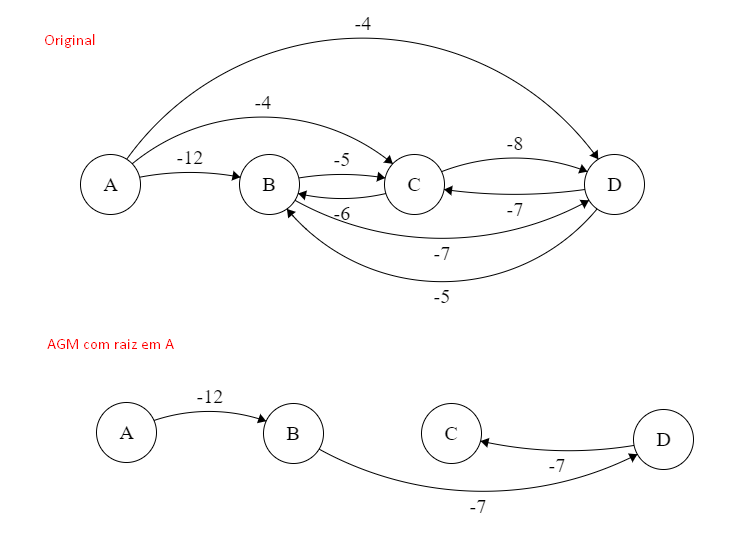
\includegraphics[width=.75\textwidth]{AGM/Exemplo 1.png}
\caption{Edmonds - Primeiro Caso de Teste}
\end{figure}

Em seguida, o método foi aplicado a um segundo grafo, desta vez com ciclos presentes, mas que não interferiram na construção da AGM. A Figura 2 fornece uma visualização do grafo e da AGM resultante, evidenciando a habilidade do algoritmo em contornar ciclos que não comprometem a estrutura da árvore geradora mínima.

\begin{figure}[ht]
\centering
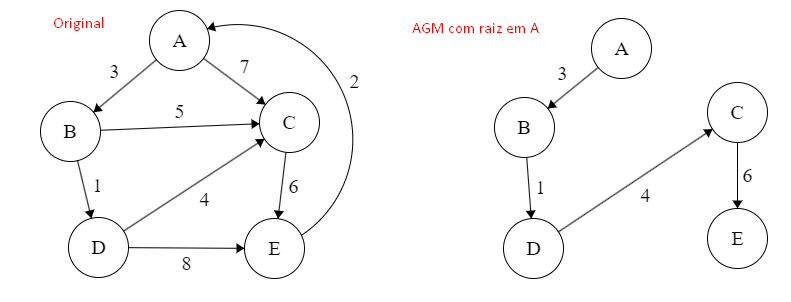
\includegraphics[width=.85\textwidth]{AGM/Exemplo 2.png}
\caption{Edmonds - Segundo Caso de Teste}
\end{figure}

O terceiro caso de teste abordou um grafo com um ciclo de três vértices, semelhante ao primeiro cenário. Os resultados indicaram que o método de Edmonds tratou corretamente esse tipo de ciclo, proporcionando uma AGM otimizada. A Figura 3 oferece uma perspectiva visual do Grafo3 e de sua respectiva AGM.

\begin{figure}[ht]
\centering
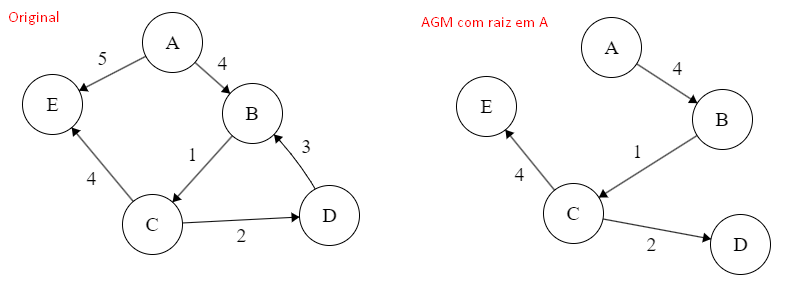
\includegraphics[width=.8\textwidth]{AGM/Exemplo 3.png}
\caption{Edmonds - Terceiro Caso de Teste}
\end{figure}

O último experimento envolveu um grafo mais simples, mas com um ciclo de quatro vértices. Novamente, o método de Edmonds foi capaz de detectar e resolver o ciclo de maneira eficaz, produzindo uma AGM com raiz no vértice \(A\). A Figura 4 ilustra esse cenário, enfatizando a qualidade do resultado obtido.

\begin{figure}[ht]
\centering
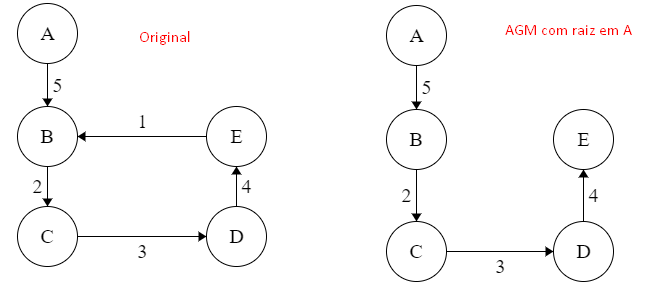
\includegraphics[width=.65\textwidth]{AGM/Exemplo 4.png}
\caption{Edmonds - Quarto Caso de Teste}
\end{figure}

Esses experimentos proporcionaram uma análise prática do desempenho do método de Edmonds em cenários diversos de grafos direcionados. 

Adicionalmente, também foi desenvolvido um método para avaliar o desempenho do algoritmo de Edmonds em diferentes tamanhos de grafos. Este método gerou grafos com uma quantidade variável de vértices, iniciando em 10 e aumentando de 10 em 10 até atingir 100 vértices. Para cada tamanho de grafo, o método de Edmonds foi executado, e o tempo de execução foi registrado. 

Utilizando a biblioteca \textit{chrono} para medição precisa do tempo, o método foi iniciado e encerrado, proporcionando uma visão detalhada do tempo necessário para encontrar a Arborescência Geradora Mínima em cada cenário. Os resultados dessas medições fornecem detalhes sobre a escalabilidade e eficiência do algoritmo em grafos de diferentes dimensões, oferecendo uma perspectiva abrangente de seu desempenho em cenários práticos.

\subsection{Tarjan}

Para os experimentos com o método de Tarjan, foram elaborados testes representativos para avaliar seu desempenho em diferentes cenários. A seguir, são descritos dois exemplos de execução do algoritmo, cada um acompanhado por um grafo ilustrativo e sua respectiva Arborescência Geradora Mínima (AGM) obtida.

O primeiro exemplo, visto na Figura 5, apresenta um grafo direcionado com oito vértices e arestas ponderadas, onde se destaca a execução do algoritmo de Tarjan. O resultado demonstra a AGM com raiz no vértice \(A\), evidenciando a eficácia do método ao lidar com grafos de diferentes tamanhos e complexidades.

\begin{figure}[ht]
\centering
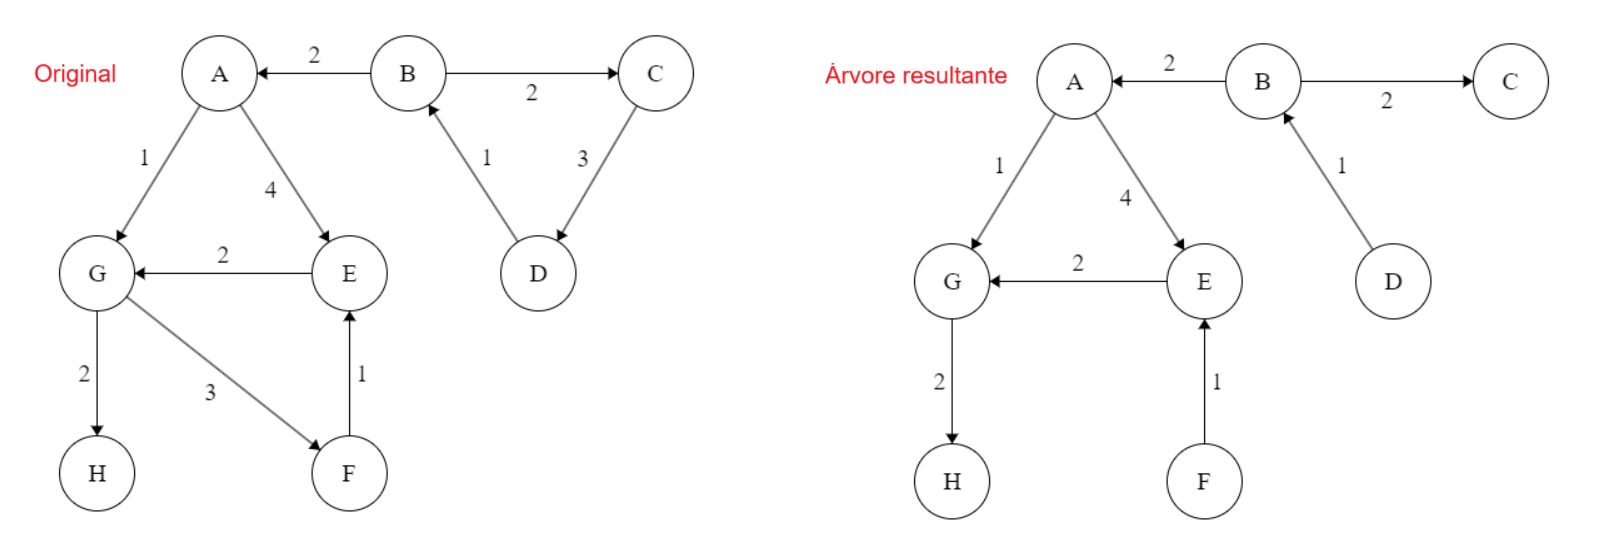
\includegraphics[width=1\textwidth]{AGM/caso1.png}
\caption{Tarjan - Primeiro Caso de Teste}
\end{figure}

Na Figura 6, a seguir, tem-se o segundo caso de teste, que utiliza um grafo direcionado menor, composto por quatro vértices e arestas ponderadas. A execução do algoritmo de Tarjan nesse cenário resulta em uma AGM, com raiz no vértice \(B\), que atende aos requisitos da Arborescência Geradora Mínima.

\begin{figure}[ht]
\centering
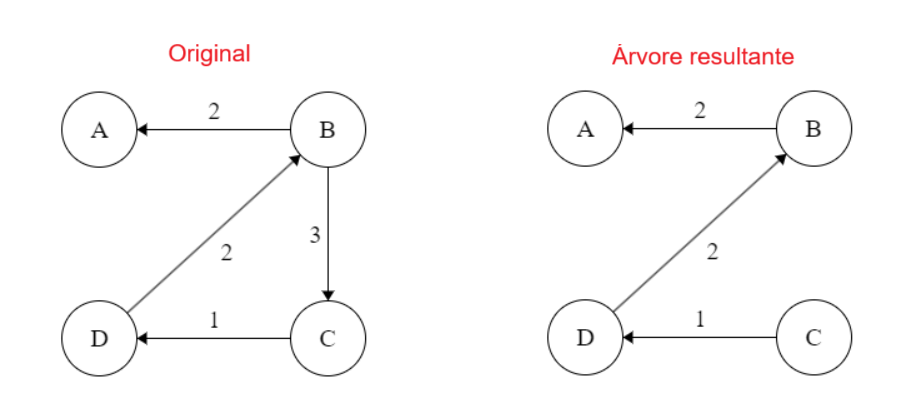
\includegraphics[width=.6\textwidth]{AGM/caso2.png}
\caption{Tarjan - Segundo Caso de Teste}
\end{figure}

Adicionalmente, para avaliar o desempenho do algoritmo em diferentes tamanhos de grafos, foram conduzidos experimentos variando o número de vértices de 10 a 100, com incrementos de 10 em cada execução. O tempo gasto para processar cada grafo foi registrado, proporcionando uma visão abrangente do comportamento do algoritmo diante de diversas instâncias, assim como o que foi feito para o algoritmo de Edmonds.

Os experimentos evidenciam a robustez e escalabilidade do algoritmo de Tarjan, destacando sua aplicabilidade em diferentes contextos e tamanhos de grafos direcionados.

\section{Resultados Obtidos}

Para explorar a relação entre o número de vértices nos grafos de teste e o tempo de execução dos algoritmos, foi conduzida uma análise abrangente do desempenho dos métodos de Edmonds e Tarjan. O experimento retornou informações relevantes sobre o comportamento de ambos os métodos em diferentes cenários.

Para o método de Edmonds, os resultados indicam que o tempo de execução aumenta proporcionalmente ao número de vértices. Notavelmente, ao considerar um grafo com 100 vértices, o algoritmo de Edmonds exigiu aproximadamente 6000 microssegundos para concluir o processamento. Cabe ressaltar que, no processo de construção dos grafos de teste, foi considerada a inclusão de uma aresta para cada combinação possível de vértices, contribuindo para uma análise abrangente da eficiência do método. Detalhes visuais dessas relações podem ser observados na Figura 7 que ilustra o impacto do tamanho do grafo no desempenho do método.

\begin{figure}[ht]
\centering
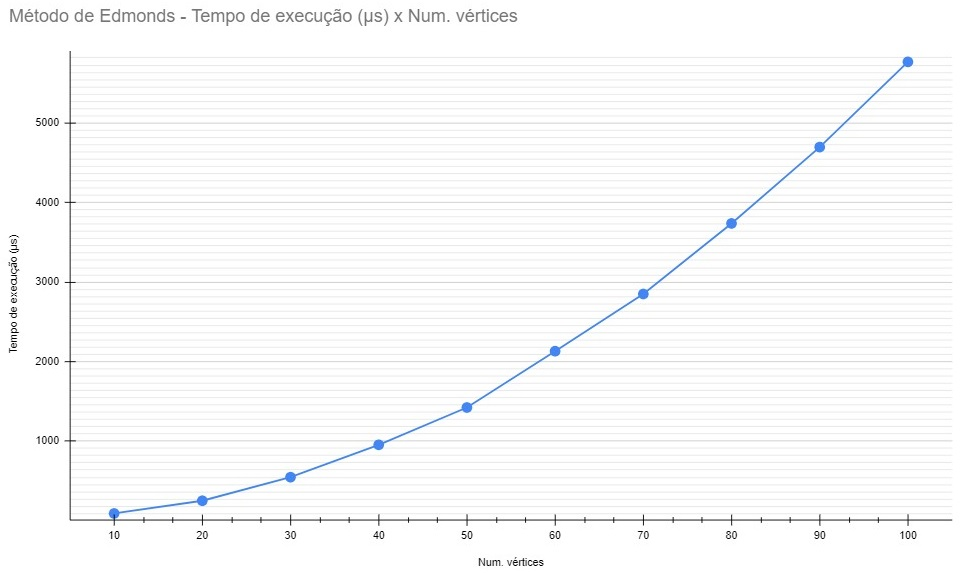
\includegraphics[width=.7\textwidth]{AGM/grafico1.jpeg}
\caption{Edmonds - Relação Vértices x Tempo de Execução}
\end{figure}

Já para o algoritmo de Tarjan, observou-se uma relação proporcional entre o tempo de execução e o número de vértices no grafo direcionado. Especificamente, ao analisar um cenário com 100 vértices, o algoritmo demandou aproximadamente 8500 microssegundos para completar o processamento. Essa variação temporal está intrinsecamente associada à escolha da representação do grafo por meio de uma matriz dinâmica. Os detalhes dessa dinâmica de desempenho podem ser visualizados na Figura 8, que oferece uma perspectiva visual do impacto do tamanho do grafo na eficiência do método.

\begin{figure}[ht]
\centering
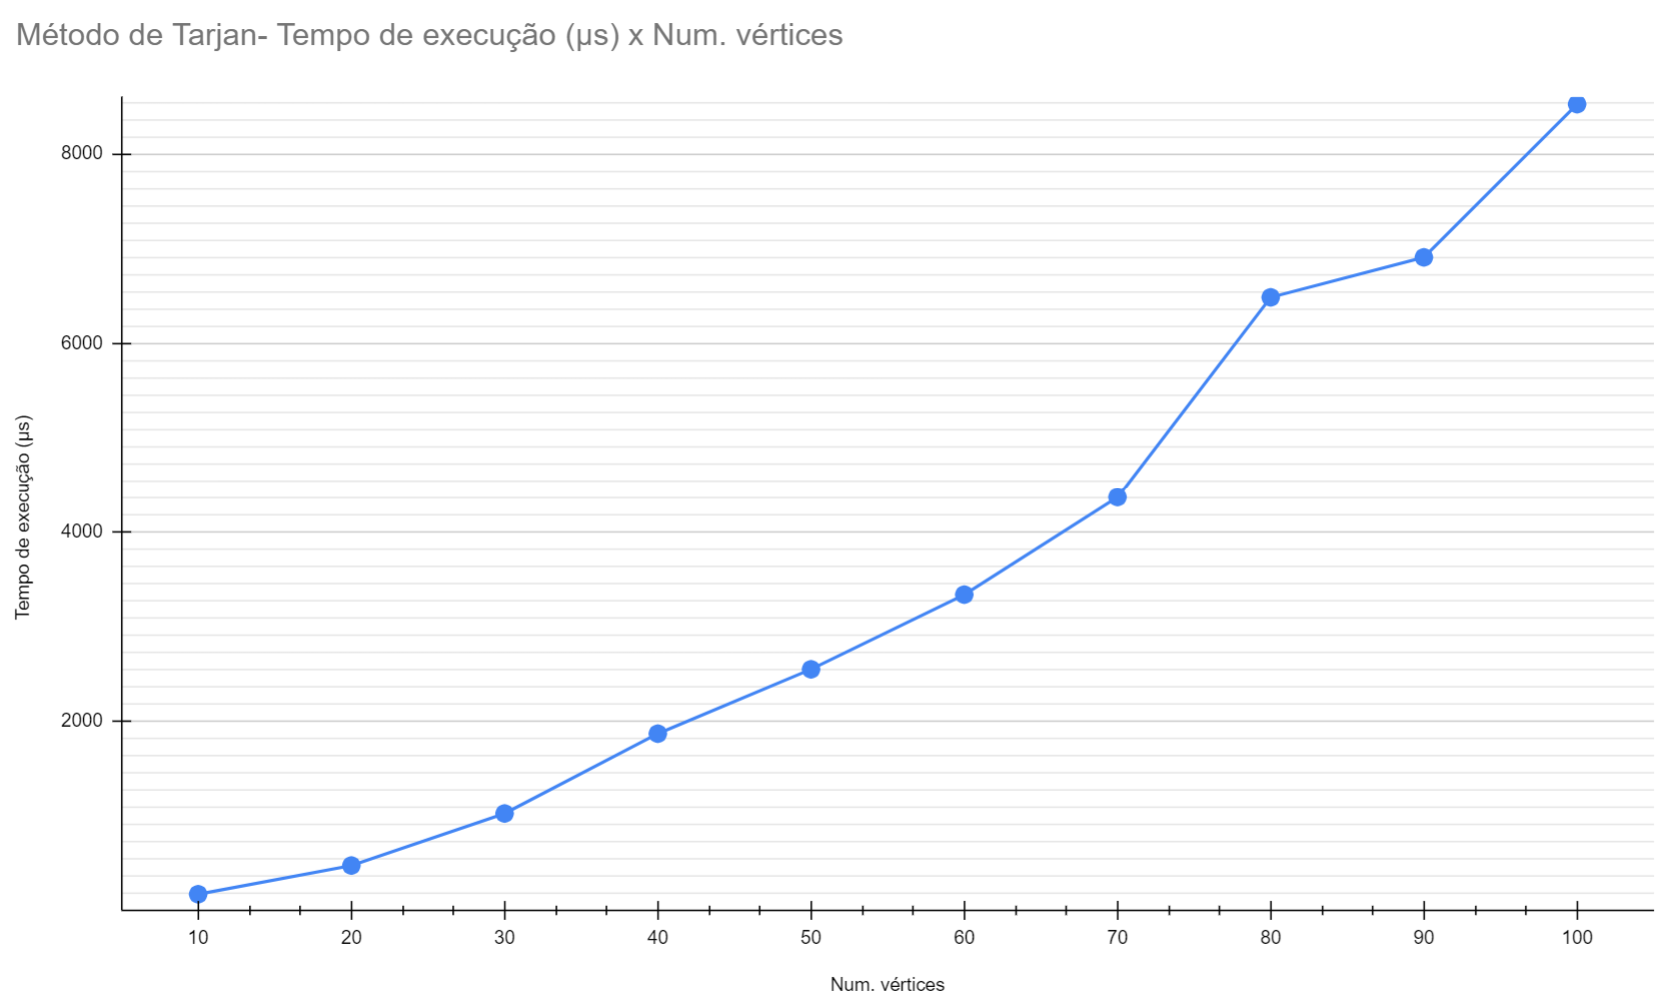
\includegraphics[width=.7\textwidth]{AGM/grafico2.png}
\caption{Tarjan - Relação Vértices x Tempo de Execução}
\end{figure}

Comparativamente, em termos de complexidade assintótica, o método de Edmonds demonstra uma complexidade \(O(nm)\), onde \(n\) representa o número de vértices e \(m\) o número de arestas. Por outro lado, o método de Tarjan apresenta uma complexidade \(O(min(n², mlogn))\) para \(n\) vértices e \(m\) arestas. Essas informações destacam nuances importantes sobre como cada algoritmo responde a grafos de diferentes tamanhos e estruturas.

Os gráficos resultantes proporcionam uma visualização clara e informativa, permitindo uma compreensão mais profunda do desempenho relativo desses métodos em diferentes cenários. Essa análise comparativa é essencial para orientar a escolha do algoritmo mais apropriado, considerando as características específicas do problema em pauta e a natureza dos grafos envolvidos.

\section{Conclusão}

Este relatório abordou dois métodos fundamentais para a resolução do problema da Arborescência Geradora Mínima (AGM) em grafos direcionados, o algoritmo de Edmonds e o algoritmo de Tarjan. O método de Edmonds, baseado em uma abordagem gulosa adaptada do algoritmo de Kruskal para grafos não direcionados, demonstrou eficácia ao construir AGMs ótimas em termos de custo. Através de experimentos, observou-se que o desempenho do algoritmo está correlacionado ao número de vértices, apresentando um aumento proporcional no tempo de execução.

Por outro lado, o algoritmo de Tarjan, inspirado na técnica de contração de ciclos, revelou-se robusto na detecção e tratamento de ciclos durante a construção da AGM. A estratégia de combinar a Busca em Profundidade (DFS) com estruturas de conjuntos disjuntos permitiu ao algoritmo de Tarjan superar desafios relacionados à presença de ciclos, resultando em AGMs eficientes e acíclicas.

Os resultados forneceram detalhes sobre o comportamento de ambos os algoritmos em grafos de diferentes tamanhos. Ao visualizar as relações entre o número de vértices e o tempo de execução, foi possível discernir nuances de desempenho e eficiência em cenários diversos. De maneira geral, este estudo contribui para a compreensão aprofundada desses métodos na solução do problema da AGM em grafos direcionados.

\bibliographystyle{sbc}
\bibliography{sbc-template}

\end{document}
